\documentclass{standalone}
\usepackage{tikz}
\usetikzlibrary{patterns, positioning}
\usepackage[sfdefault]{ClearSans} %% option 'sfdefault' activates Clear Sans as the default text font
\usepackage[T1]{fontenc}

\begin{document}
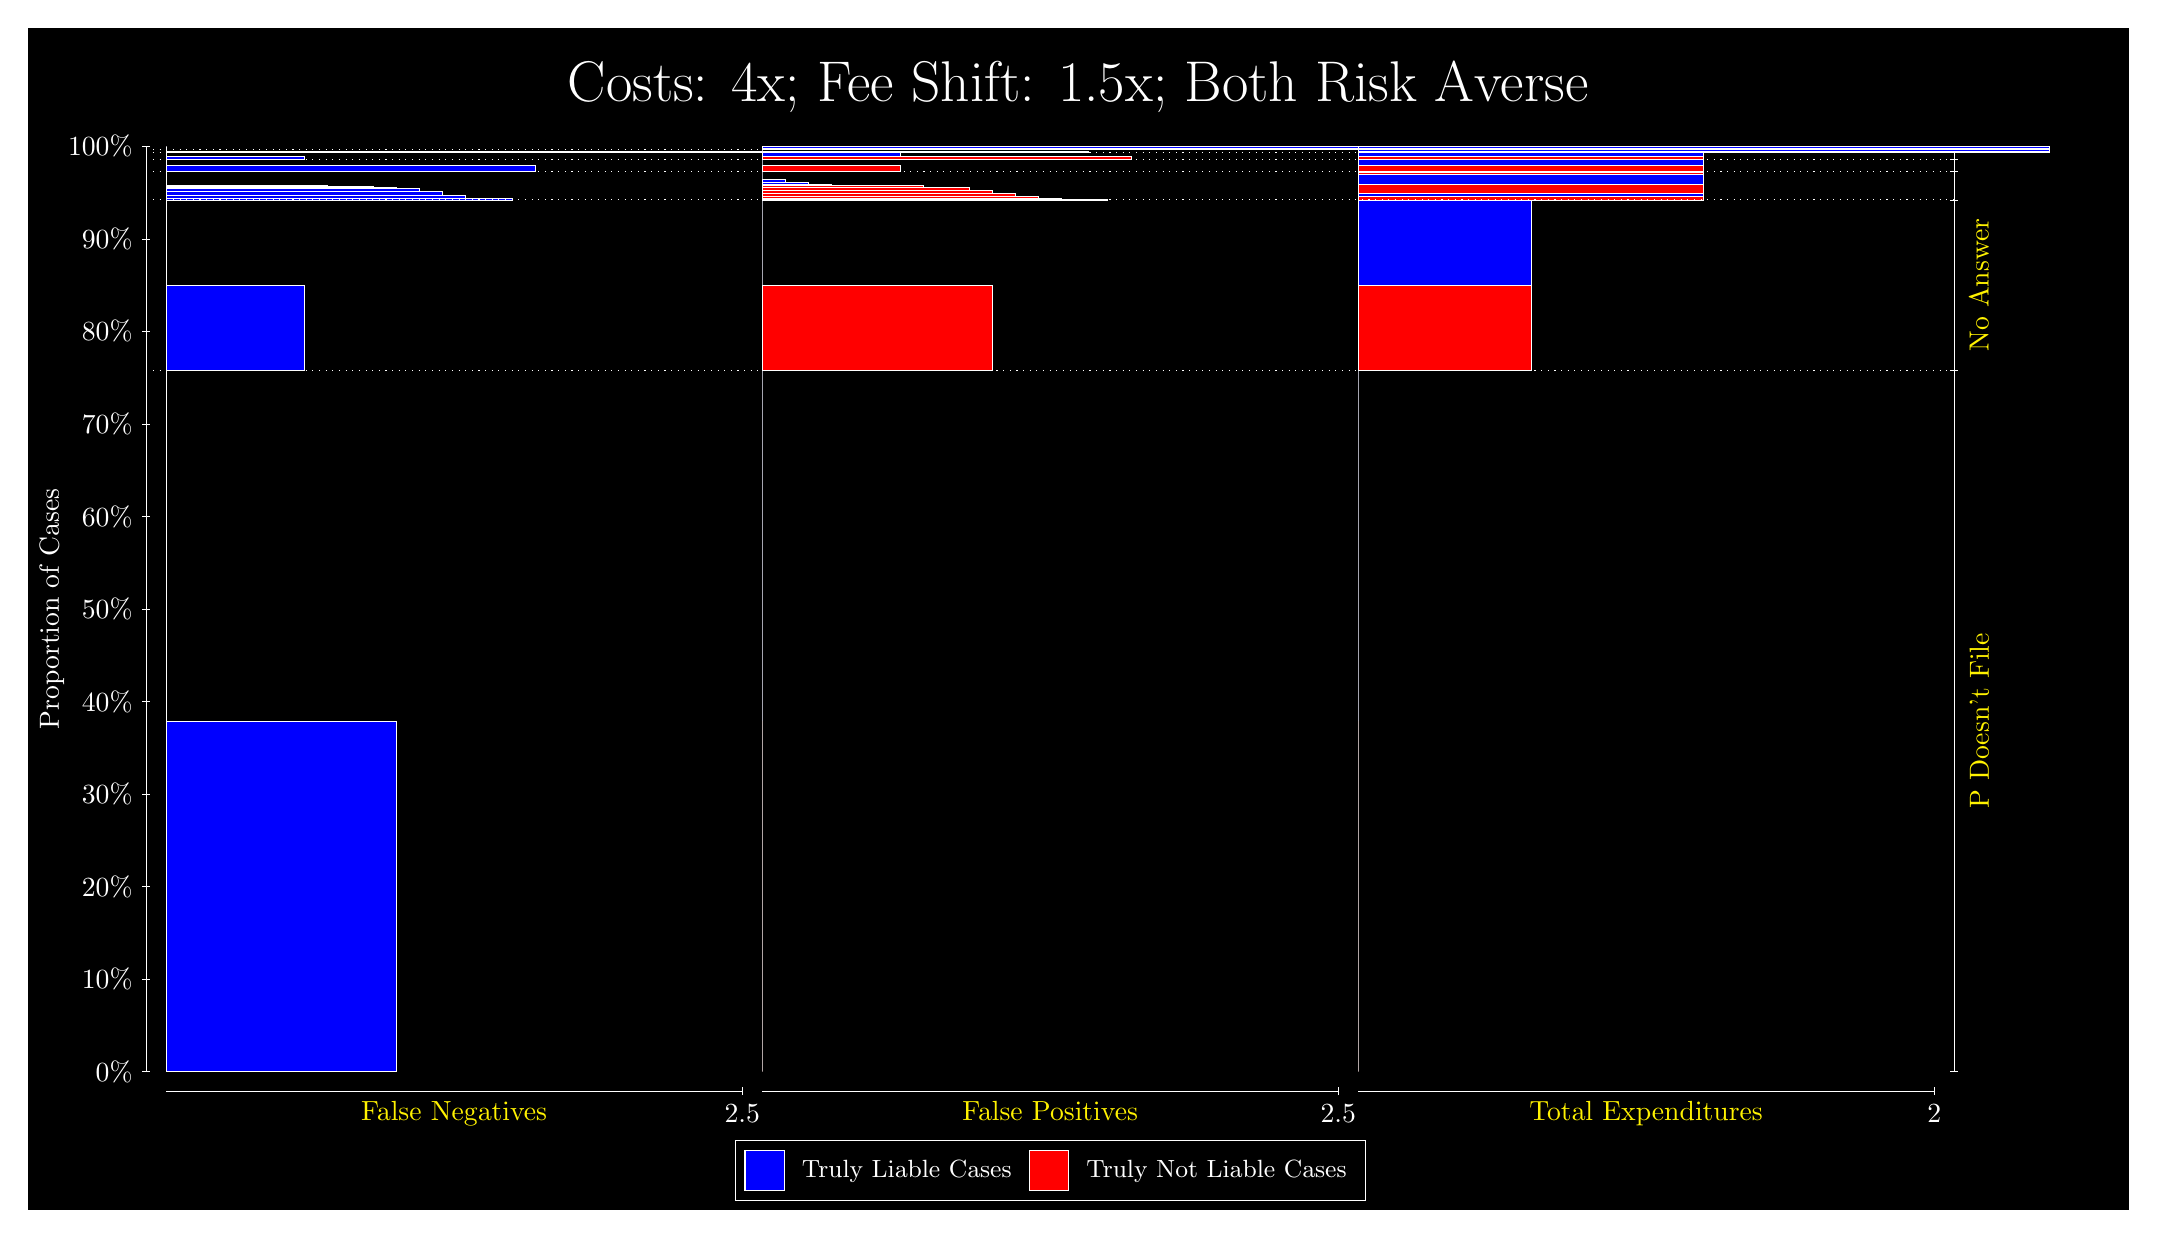
\begin{tikzpicture}
\draw[fill=black] (0,0) rectangle (26.667,15);
\draw[text=white] (0,13.5) rectangle (26.667,15) node[midway] {\huge Costs: 4x; Fee Shift: 1.5x; Both Risk Averse};
\draw[white, very thin] (1.5,1.75) -- (1.5,13.5);
\node[rotate=90, text=white, anchor=center] at (0.3, 7.625) {Proportion of Cases};
\draw[white, very thin] (1.45,1.75) -- (1.55,1.75);
\node[text=white, anchor=east] at (1.45, 1.75) {0\%};
\draw[white, very thin] (1.45,2.925) -- (1.55,2.925);
\node[text=white, anchor=east] at (1.45, 2.925) {10\%};
\draw[white, very thin] (1.45,4.1) -- (1.55,4.1);
\node[text=white, anchor=east] at (1.45, 4.1) {20\%};
\draw[white, very thin] (1.45,5.275) -- (1.55,5.275);
\node[text=white, anchor=east] at (1.45, 5.275) {30\%};
\draw[white, very thin] (1.45,6.45) -- (1.55,6.45);
\node[text=white, anchor=east] at (1.45, 6.45) {40\%};
\draw[white, very thin] (1.45,7.625) -- (1.55,7.625);
\node[text=white, anchor=east] at (1.45, 7.625) {50\%};
\draw[white, very thin] (1.45,8.8) -- (1.55,8.8);
\node[text=white, anchor=east] at (1.45, 8.8) {60\%};
\draw[white, very thin] (1.45,9.975) -- (1.55,9.975);
\node[text=white, anchor=east] at (1.45, 9.975) {70\%};
\draw[white, very thin] (1.45,11.15) -- (1.55,11.15);
\node[text=white, anchor=east] at (1.45, 11.15) {80\%};
\draw[white, very thin] (1.45,12.325) -- (1.55,12.325);
\node[text=white, anchor=east] at (1.45, 12.325) {90\%};
\draw[white, very thin] (1.45,13.5) -- (1.55,13.5);
\node[text=white, anchor=east] at (1.45, 13.5) {100\%};

\draw[white, very thin] (24.457,1.75) -- (24.457,13.5);
\draw[white, very thin] (24.407,1.75) -- (24.507,1.75);
\node[anchor=west] at (24.407, 1.75) {};
\draw[white, very thin] (24.407,10.655) -- (24.507,10.655);
\node[anchor=west] at (24.407, 10.655) {};
\draw[white, very thin] (24.407,12.821) -- (24.507,12.821);
\node[anchor=west] at (24.407, 12.821) {};
\draw[white, very thin] (24.407,13.182) -- (24.507,13.182);
\node[anchor=west] at (24.407, 13.182) {};
\draw[white, very thin] (24.407,13.332) -- (24.507,13.332);
\node[anchor=west] at (24.407, 13.332) {};
\draw[white, very thin] (24.407,13.42) -- (24.507,13.42);
\node[anchor=west] at (24.407, 13.42) {};
\draw[white, very thin] (24.407,13.46) -- (24.507,13.46);
\node[anchor=west] at (24.407, 13.46) {};
\draw[white, very thin] (24.407,13.5) -- (24.507,13.5);
\node[anchor=west] at (24.407, 13.5) {};

\draw[white, very thin, fill=blue] (1.75,1.75) rectangle (4.6775,6.2024);
\draw[white, very thin, fill=red] (1.75,6.2024) rectangle (1.75,10.655);
\draw[white, very thin, fill=blue] (1.75,10.655) rectangle (3.5065,11.738);
\draw[white, very thin, fill=red] (1.75,11.738) rectangle (1.75,12.821);
\draw[white, very thin, fill=blue] (1.75,12.821) rectangle (6.1413,12.837);
\draw[white, very thin, fill=blue] (1.75,12.837) rectangle (5.8486,12.845);
\draw[white, very thin, fill=blue] (1.75,12.845) rectangle (5.5558,12.881);
\draw[white, very thin, fill=blue] (1.75,12.881) rectangle (5.2631,12.924);
\draw[white, very thin, fill=blue] (1.75,12.924) rectangle (4.9703,12.964);
\draw[white, very thin, fill=blue] (1.75,12.964) rectangle (4.6775,12.981);
\draw[white, very thin, fill=blue] (1.75,12.981) rectangle (4.3848,12.992);
\draw[white, very thin, fill=blue] (1.75,12.992) rectangle (4.092,12.998);
\draw[white, very thin, fill=blue] (1.75,12.998) rectangle (3.7993,13.003);
\draw[white, very thin, fill=red] (1.75,13.003) rectangle (1.75,13.182);
\draw[white, very thin, fill=blue] (1.75,13.182) rectangle (6.4341,13.256);
\draw[white, very thin, fill=red] (1.75,13.256) rectangle (1.75,13.332);
\draw[white, very thin, fill=blue] (1.75,13.332) rectangle (3.5065,13.376);
\draw[white, very thin, fill=red] (1.75,13.376) rectangle (1.75,13.42);
\draw[white, very thin, fill=blue] (1.75,13.42) rectangle (13.46,13.438);
\draw[white, very thin, fill=red] (1.75,13.438) rectangle (1.75,13.46);
\draw[white, very thin, fill=red] (1.75,13.46) rectangle (1.75,13.479);
\draw[white, very thin, fill=blue] (1.75,13.479) rectangle (1.75,13.5);
\draw[white, very thin, fill=red] (9.3189,1.75) rectangle (9.3189,6.2024);
\draw[white, very thin, fill=blue] (9.3189,6.2024) rectangle (9.3189,10.655);
\draw[white, very thin, fill=red] (9.3189,10.655) rectangle (12.246,11.739);
\draw[white, very thin, fill=blue] (9.3189,11.739) rectangle (9.3189,12.821);
\draw[white, very thin, fill=red] (9.3189,12.821) rectangle (13.71,12.826);
\draw[white, very thin, fill=red] (9.3189,12.826) rectangle (13.417,12.832);
\draw[white, very thin, fill=red] (9.3189,12.832) rectangle (13.125,12.843);
\draw[white, very thin, fill=red] (9.3189,12.843) rectangle (12.832,12.86);
\draw[white, very thin, fill=red] (9.3189,12.86) rectangle (12.539,12.899);
\draw[white, very thin, fill=red] (9.3189,12.899) rectangle (12.246,12.942);
\draw[white, very thin, fill=red] (9.3189,12.942) rectangle (11.954,12.976);
\draw[white, very thin, fill=red] (9.3189,12.976) rectangle (11.661,12.984);
\draw[white, very thin, fill=red] (9.3189,12.984) rectangle (11.368,13.001);
\draw[white, very thin, fill=blue] (9.3189,13.001) rectangle (10.783,13.006);
\draw[white, very thin, fill=blue] (9.3189,13.006) rectangle (10.49,13.011);
\draw[white, very thin, fill=blue] (9.3189,13.011) rectangle (10.197,13.023);
\draw[white, very thin, fill=blue] (9.3189,13.023) rectangle (9.9044,13.039);
\draw[white, very thin, fill=blue] (9.3189,13.039) rectangle (9.6116,13.08);
\draw[white, very thin, fill=blue] (9.3189,13.08) rectangle (9.3189,13.182);
\draw[white, very thin, fill=red] (9.3189,13.182) rectangle (11.075,13.258);
\draw[white, very thin, fill=blue] (9.3189,13.258) rectangle (9.3189,13.332);
\draw[white, very thin, fill=red] (9.3189,13.332) rectangle (14.003,13.376);
\draw[white, very thin, fill=blue] (9.3189,13.376) rectangle (11.075,13.42);
\draw[white, very thin, fill=red] (9.3189,13.42) rectangle (9.3189,13.442);
\draw[white, very thin, fill=blue] (9.3189,13.442) rectangle (9.3189,13.46);
\draw[white, very thin, fill=red] (9.3189,13.46) rectangle (21.029,13.479);
\draw[white, very thin, fill=blue] (9.3189,13.479) rectangle (18.102,13.5);
\draw[white, very thin, fill=red] (16.888,1.75) rectangle (16.888,6.2024);
\draw[white, very thin, fill=blue] (16.888,6.2024) rectangle (16.888,10.655);
\draw[white, very thin, fill=red] (16.888,10.655) rectangle (19.083,11.739);
\draw[white, very thin, fill=blue] (16.888,11.739) rectangle (19.083,12.821);
\draw[white, very thin, fill=red] (16.888,12.821) rectangle (21.279,12.861);
\draw[white, very thin, fill=blue] (16.888,12.861) rectangle (21.279,12.901);
\draw[white, very thin, fill=red] (16.888,12.901) rectangle (21.279,13.024);
\draw[white, very thin, fill=blue] (16.888,13.024) rectangle (21.279,13.148);
\draw[white, very thin, fill=red] (16.888,13.148) rectangle (21.279,13.165);
\draw[white, very thin, fill=blue] (16.888,13.165) rectangle (21.279,13.182);
\draw[white, very thin, fill=red] (16.888,13.182) rectangle (21.279,13.258);
\draw[white, very thin, fill=blue] (16.888,13.258) rectangle (21.279,13.332);
\draw[white, very thin, fill=red] (16.888,13.332) rectangle (21.279,13.376);
\draw[white, very thin, fill=blue] (16.888,13.376) rectangle (21.279,13.42);
\draw[white, very thin, fill=red] (16.888,13.42) rectangle (25.67,13.442);
\draw[white, very thin, fill=blue] (16.888,13.442) rectangle (25.67,13.46);
\draw[white, very thin, fill=red] (16.888,13.46) rectangle (25.67,13.479);
\draw[white, very thin, fill=blue] (16.888,13.479) rectangle (25.67,13.5);
\draw[white, dotted] (1.5,10.655) -- (24.457,10.655);
\draw[white, dotted] (1.5,12.821) -- (24.457,12.821);
\draw[white, dotted] (1.5,13.182) -- (24.457,13.182);
\draw[white, dotted] (1.5,13.332) -- (24.457,13.332);
\draw[white, dotted] (1.5,13.42) -- (24.457,13.42);
\draw[white, dotted] (1.5,13.46) -- (24.457,13.46);
\draw[white, very thin] (1.75,1.5) -- (9.0689,1.5);
\node[text=yellow, anchor=north] at (5.4094, 1.5) {False Negatives};
\draw[white, very thin] (9.0689,1.45) -- (9.0689,1.55);
\node[text=white, anchor=north] at (9.0689, 1.45) {2.5};

\draw[white, very thin] (9.3189,1.5) -- (16.638,1.5);
\node[text=yellow, anchor=north] at (12.978, 1.5) {False Positives};
\draw[white, very thin] (16.638,1.45) -- (16.638,1.55);
\node[text=white, anchor=north] at (16.638, 1.45) {2.5};

\draw[white, very thin] (16.888,1.5) -- (24.207,1.5);
\node[text=yellow, anchor=north] at (20.547, 1.5) {Total Expenditures};
\draw[white, very thin] (24.207,1.45) -- (24.207,1.55);
\node[text=white, anchor=north] at (24.207, 1.45) {2};

\node[text=yellow, centered, rotate=90] at (24.777, 6.2024) {P Doesn't File};
\node[text=yellow, centered, rotate=90] at (24.777, 11.738) {No Answer};






\draw (12.978300999999998,1.5) node[draw=none] (baseCoordinate) {};
\begin{scope}[align=center]
        \matrix[scale=0.5, draw=white, below=0.5cm of baseCoordinate, nodes={draw}, column sep=0.1cm]{
            \node[rectangle, draw, minimum width=0.5cm, minimum height=0.5cm, fill=blue] {}; &
            \node[draw=none, font=\small, text=white] (B) {Truly Liable Cases}; &
            \node[rectangle, draw, minimum width=0.5cm, minimum height=0.5cm, fill=red] {}; &
            \node[draw=none, font=\small, text=white] (B) {Truly Not Liable Cases}; \\
            };
\end{scope}

\end{tikzpicture}
\end{document}